\chapter{Landslide}
\inspirationalquote{Somewhere is the promise of an uncharted trail, with 700 branching limbs and 700 ways to fail.}
{ThouShaltNot, "Cardinal Directions"}

Landslide is a model checker implemented as a plug-in module for x86 full-system simulators.
The program to be tested runs in a simulated environment,
and Landslide uses its access to the simulator's internal state to inspect and manipulate the memory and thread scheduling of the program as it executes.
As of this thesis's writing, Landslide supports the use of two possible simulators:

\begin{itemize}
	\item {\bf Simics} \cite{simics}, a proprietary simulator licensed commercially by Wind River, used at CMU in 15-410 to run Pebbles thread libraries and kernels, and
	\item {\bf Bochs} \cite{bochs}, an open-source (LGPL) simulator used at the University of Chicago, Berkeley, and other schools to run Pintos kernels.
\end{itemize}

% TODO: update this linkerino (repository name)
% TODO: add some backup linkeroos
The Bochs port of Landslide is likewise open-source and available at \url{https://github.com/bblum/bochs}.
% TODO: refresh
The HEAD commit at the time of writing is 8984021.
The Simics port uses Simics's proprietary API and is hence unlicensed and available upon request for educational use only.

This chapter will discuss Landslide's outer and inner workings in all their gory detail.
It is intended for the aspiring developer or the ambitious user
and hence unlike other chapters is written in the style of documentation rather than as a report of research results.

%%%%%%%%%%%%%%%%%%%%%%%%%%%%%%%%%%%%%%%%%%%%%%%%%%%%%%%%%%%%%%%%%%%%%%%%%%%%%%%%
%%%%%%%%%%%%%%%%%%%%%%%%%%%%%%%%%%%%%%%%%%%%%%%%%%%%%%%%%%%%%%%%%%%%%%%%%%%%%%%%
%%%%%%%%%%%%%%%%%%%%%%%%%%%%%%%%%%%%%%%%%%%%%%%%%%%%%%%%%%%%%%%%%%%%%%%%%%%%%%%%

\section{User interface}

This section describes the features of Landslide the average student user should expect to interact with.
% TODO: make more specific section reference
Separate user guides also exist, described in Chapter~\ref{chap:410}.

%%%%%%%%%%%%%%%%%%%%%%%%%%%%%%%%%%%%%%%%%%%%%%%%%%%%%%%%%%%%%%%%%%%%%%%%%%%%%%%%

\subsection{Setup}

Two setup scripts are provided, one for each supported kernel architecture: {\tt p2-setup.sh} and {\tt pintos-setup.sh}.
The user should supply the directory containing their project implementation.
The latter script also supports arguments specifying which of the Pintos projects to target.
For example:
\begin{itemize}
	\item {\tt ./p2-setup.sh /path/to/my/p2}
	\item {\tt ./pintos-setup.sh /path/to/my/threads} (2nd argument defaults to ``{\tt threads}'')
	\item {\tt ./pintos-setup.sh /path/to/my/userprog userprog}
\end{itemize}

These scripts accomplish the following setup tasks (among other trivialities):
\begin{itemize}
	\item Copy the user's code into {\tt pebsim/p2-basecode/} or {\tt pebsim/pintos/},
		which contain a pre-annotated Pebbles reference kernel binary or pre-annotated Pintos basecode, respectively.
	\item Build the code in its new location.
	\item Run the instrumentation script on the resulting binary to let Landslide know where all the important functions are
		(see \sect{\ref{sec:landslide-glue}}).
\end{itemize}

%%%%%%%%%%%%%%%%%%%%%%%%%%%%%%%%%%%%%%%%%%%%%%%%%%%%%%%%%%%%%%%%%%%%%%%%%%%%%%%%

\subsection{Running Landslide through Quicksand}
\label{sec:landslide-quicksand-options}

The preferred method of invoking Landslide is through Quicksand, the Iterative Deepening wrapper program which has all of Chapter~\ref{chap:quicksand} to itself.
% TODO: add quicksand symlink
This is done via the {\tt ./landslide} script in the top-level directory, which:
\begin{itemize}
	\item Checks if the user needs to run {\tt *-setup.sh} again, in case their source code was more recently updated than the existing annotated build (a common mistake),
	\item Passes its arguments through to {\tt id/landslide-id}, the Quicksand binary,
		and
	\item (If during the student user study,) compresses the resulting log files,
		creates a snapshot tarball of them and the current version of the user's code,
		and sends it to me for nefarious research purposes.
\end{itemize}

%%%%%%%%%%%%%%%%%%%%%%%%%%%%%%%%%%%%%%%%%%%%%%%%%%%%%%%%%%%%%%%%%%%%%%%%%%%%%%%%

\subsubsection{Command-line argments}

The following command line arguments are recommended for the common user.

\begin{itemize}
	\item {\tt -p PROGRAM}: the name of the test case to invoke
	\item {\tt -t TIME}: wall-clock time limit, in seconds; or suffixed with one of {\tt ydhms} for years, days, hours, minutes, or seconds respectively (default 1h)
	\item {\tt -c CPUS}: maximum number of Landslide instances to run in parallel (defaults to half the number of system CPUs)
	\item {\tt -i INTERVAL}: interval of time between printing progress reports (default 10s)
	\item {\tt -d TRACEDIR}: directory for resulting bug traces (default current directory)
	\item {\tt -v}: verbose mode (issues output for each executed interleaving by each instance of landslide, makes progress reports more detailed, etc)
	\item {\tt -l}: leave Landslide log files from completed state spaces even when no bug was found (deleted automatically by default)
	\item {\tt -h}: print help text and exit immediately
\end{itemize}

The following ``secret'' arguments also exist, primarily for my own use in running experiments or debugging.

\begin{itemize}
	\item {\tt -C}: enable ``control experiment'' mode, i.e., run only 1 instance of Landslide, with all (non-data-race) preemption points enabled in advance
		% TODO: put a section reference here
	\item {\tt -I}: enable Iterative Context Bounding (requires {\tt -C}, although future work may relax this restriction);
		this generally causes bugs to be found faster should they exist, but degrades completion time
		(\sect{\ref{sec:landslide-icb}})
	\item {\tt -0}: enable Preempt-Everywhere mode (\sect{\ref{sec:quicksand-eval}}, requires {\tt -C})
	\item {\tt -H}: use Limited Happens-Before for data-race analysis (\sect{\ref{sec:background-hb}})
		(default for Pebbles kernelspace mode)
	\item {\tt -V}: use vector-clock-based Pure Happens-Before for data-race analysis (\sect{\ref{sec:background-hb}})
		(default for P2 userspace and Pintos modes)
	\item {\tt -X}: support transactional memory (Chapter~\ref{chap:tm})
		% TODO: make a more specific section reference
	\item {\tt -A}: support multiple abort codes during transaction failure (Chapter~\ref{chap:tm});
		required for testing programs which behave differently under different abort circumstances,
		but impacts the state space size
	\item {\tt -P}: support Pintos architecture (enabled automatically when {\tt pintos-setup.sh} is run)
	\item {\tt -4}: support Pebbles architecture (enabled automatically when {\tt p2-setup.sh} is run)
		% TODO: put a section reference
	\item {\tt -e ETAFACTOR}: configure heuristic state space ETA deferring factor (described in detail in {\tt id/option.c})
	\item {\tt -E ETATHRESH}: configure heuristic threshold of state space progress for judging ETA stability (described in detail in {\tt id/option.c})
\end{itemize}

Quicksand will automatically generate configuration files and invoke Landslide according to the process described in the next section.

%%%%%%%%%%%%%%%%%%%%%%%%%%%%%%%%%%%%%%%%%%%%%%%%%%%%%%%%%%%%%%%%%%%%%%%%%%%%%%%%

\subsection{Running Landslide directly}
\label{sec:landslide-directly}

Rather than letting Quicksand juggle multiple instances of Landslide,
the user may run a single instance directly, optionally configuring the preemption points by hand.
This is recommended only for enthusiastic users who are annotating their own kernel.

The script {\tt pebsim/landslide} invokes Landslide thus.
It should be run from within the {\tt pebsim/} directory.
When supplied no arguments, it reads configuration options from {\tt pebsim/config.landslide}
(a bash script expected to define certain variables as described in \sect{\ref{sec:landslide-glue}}).
The user may optionally specify a file containing additional config directives
% , such as custom preemption points,
as an argument.\footnote{
Quicksand actually supplies two such files as arguments: one ``static'' config file and one ''dynamic'' config file.
The former contains options which require recompiling Landslide (e.g., whether or not to use ICB is controlled by an {\tt \#ifdef} in Landslide's code),
while the latter contains options which Landslide interprets at runtime (e.g., which preemption points to use).
The static options do not change between Landslide instances in a single Quicksand run,
avoiding long Landslide start-up times.
}
Such supported options are as follows.

\subsubsection{Dynamic configuration options}
\label{sec:landslide-dynamicconfig}

First, the following options may be changed without triggering a recompile of Landslide.
They are implemented as bash functions defined in {\tt pebsim/build.sh}.

\begin{itemize}
	\item {\tt within\_function FUNC} - adds {\tt FUNC} to a whitelist of functions required to appear in the current stack trace before identifying a preemption point (see \sect{\ref{sec:landslide-pps}})
	\item {\tt without\_function FUNC} - as above, but a blacklist instead of a whitelist
	\item {\tt within\_user\_function FUNC} - as two above but finds the function in the userspace test program rather than the kernel code.
	\item {\tt without\_user\_function FUNC} - difference to two above same as stated one above.
	\item {\tt data\_race ADDR TID LAST\_CALL CURRENT\_SYSCALL} - specifies a data-race preemption point.
		\begin{itemize}
			\item {\tt ADDR} shall be the code address (in hex) of the racing address,
			{\em before} the execution of which a preemption will be issued.
			\item {\tt TID} indicates a thread ID required to be running for this data race.
				To specify data race PPs across all threads at once, set {\tt FILTER\_DRS\_BY\_TID=0} (see next section).
			\item {\tt LAST\_CALL} indicates a code address required to be the site of the last {\tt call} instruction executed
				(similar to specifying a stack trace, but using a full stack trace here degrades performance too much),
				or 0 to not use this feature.
				From personal experience I found this option rather useless and recommend always supplying 0.
				% TODO: fix this section ref
				For further discussion see \sect{\ref{sec:quicksand-pps}}.
			\item {\tt CURRENT\_SYSCALL} indicates the system call number if a user-space data race comes from within a kernel system call which accesses user memory (Pebbles only).
				Usually 0 (i.e., not in kernel code) but {\tt deschedule}'s system call number is common as well.
		\end{itemize}
	\item {\tt input\_pipe FILENAME} - FIFO file used for receiving messages from Quicksand (e.g. to suspend or resume execution).
		Requires {\tt id\_magic} option to be set (next section below).
		The odds that a human user will find spiritual enlightenment through using this option by hand are infinitesimal.
	\item {\tt output\_pipe FILENAME} - as above but for sending messages.
\end{itemize}

\subsubsection{Static configuration options}
\label{sec:landslide-staticconfig}

Next, configuration options which affect an {\tt \#ifdef} in Landslide and will trigger a recompile upon changing.
%These span a wide variety of features, sorted below in subsections by roughly how interesting I think they are.
Unless otherwise specified these are boolean flags (1 or 0) and the example value shown indicates the default used if unspecified.

\begin{itemize}
\item {\bf Search algorithm options}
\begin{itemize}
	\item {\tt ICB=0} - enable Iterative Context Bounding (\sect{\ref{sec:landslide-icb}});
		corresponds to {\tt -I} in \sect{\ref{sec:landslide-quicksand-options}}.
	\item {\tt PREEMPT\_EVERYWHERE=0} - enable Preempt-Everywhere mode (\sect{\ref{sec:quicksand-eval}});
		corresponds to {\tt -0} in \sect{\ref{sec:landslide-quicksand-options}}.
	\item {\tt EXPLORE\_BACKWARDS=0} - configure whether, at each newly encountered preemption point,
		to allow the current thread to run first then later upon backtracking to preempt (0),
		or to issue preemptions first and then try continuing the current thread later (1).
		0 tends to produce shorter preemption traces while 1 tends to find bugs faster (\cite{landslide} \S{}8.7.1).
		Not compatible with ICB.
\end{itemize}

\item {\bf Memory analysis options}
\begin{itemize}
	\item {\tt PURE\_HAPPENS\_BEFORE=1} - select Pure Happens-Before (1) or Limited Happens-Before (2) (\sect{\ref{sec:background-hb}});
		corresponds to {\tt -V}/{\tt -H} in \sect{\ref{sec:landslide-quicksand-options}}.
	\item {\tt FILTER\_DRS\_BY\_TID=1} - configures whether to use the {\tt TID} parameter of {\tt data\_\allowbreak{}race} described above.
	\item {\tt FILTER\_DRS\_BY\_LAST\_CALL=0} - configures whether to use the {\tt LAST\_CALL} parameter of {\tt data\_race} described above.
	\item {\tt ALLOW\_LOCK\_HANDOFF=0} - configures lockset tracking to permit or disallow a lock taken by one thread to be released by another thread.%
		\footnote{If enabled, accesses performed by the second thread before unlocking will not be considered protected by that lock,
			as Landslide cannot infer what prior event abstractly represented the lock's ownership changing,
			leading to spurious data race reports.
			This could be solved in future work with a new annotation.}
	\item {\tt ALLOW\_REENTRANT\_MALLOC\_FREE=0} - allow two threads to be in {\tt malloc}, {\tt free}, or so on simultaneously without declaring it a bug.%
		\footnote{Used in Pintos, where those functions lock/unlock the heap mutex themselves rather than relying on a wrapper function to do so before invoking them.}
	\item {\tt TESTING\_MUTEXES=0} - configure ``mutex testing'' mode (1),
		in which the data race analysis will not consider a mutex's implementation to be protected by the mutex itself.
		In other words, the mutex's internal memory accesses will be flagged as data races,
		thereby enabling Landslide to verify the mutual exclusion property.
		Normally (0), Landslide assumes mutual exclusion is provided in order to efficiently find data races in the rest of the code.
		Quicksand will automatically set this option for P2s when {\tt -t mutex\_test} is specified.
\end{itemize}

\item {\bf Interface options}
\begin{itemize}
	\item {\tt TEST\_CASE=NAME} - configure the name of the test program to run (mandatory; no default)
	\item {\tt VERBOSE=0} - enable more verbose output
	\item {\tt BREAK\_ON\_BUG=0} - configure whether to exit the simulator or drop into a debug prompt when a bug is found. Simics only and not compatible with Quicksand.
	\item {\tt DONT\_EXPLORE=0} - if enabled, Landslide will not perform stateless model checking but rather will execute the default thread interleaving then exit (useful for manual inspection of preemption points).
	\item {\tt PRINT\_DATA\_RACES=0} - as it says on the tin (for stand-alone use; will message them to Quicksand regardless).
	\item {\tt TABULAR\_TRACE=1} - configure whether to emit bug reports to the console (0) or to an HTML trace file (1)
\end{itemize}
\end{itemize}

%%%%%%%%%%%%%%%%%%%%%%%%%%%%%%%%%%%%%%%%%%%%%%%%%%%%%%%%%%%%%%%%%%%%%%%%%%%%%%%%

\subsection{Bug reports}
\label{sec:landslide-bugreport}

When Landslide finds a bug, it produces an execution trace of the particular interleaving of threads that led to the bug.
This takes the form of a two-dimensional table,
with a column for each thread,
and each row representing the continuous execution of one thread between two (not necessarily consecutive) preemption points.
In each row, the cell in the column corresponding to the executed thread will contain a stack trace,
indicating the code location of the preemption point {\em at the end} of that thread transition
(i.e., each stack trace indicates ``this thread ran until it reached the indicated line of code'').
The bug reports are formatted in html, recommended to be viewed in a web browser.
An example is shown in Figure~\ref{fig:bugreport}.

In addition to the preemption trace, the bug report provides some additional helpful information:
a stack trace of the current thread at the ultimate point when the bug was executed,
a message indicating the nature of the bug encountered,
statistics about the size of the state space,
and optionally additional information about the bug.%
\footnote{For certain types of bugs, not pictured here;
for example, use-after-frees will report separate stack traces
indicating when the corresponding heap block was last allocated and freed.
The intrepid source-diver may find all such cases of extra bug details
by searching for the macro {\tt FOUND\_A\_BUG\_HTML\_INFO} in Landslide's code.}


% TODO: check figure placement
\begin{figure}[t]
	\begin{center}
		% nb. generated from landslide-trace-1506524837.14.html
		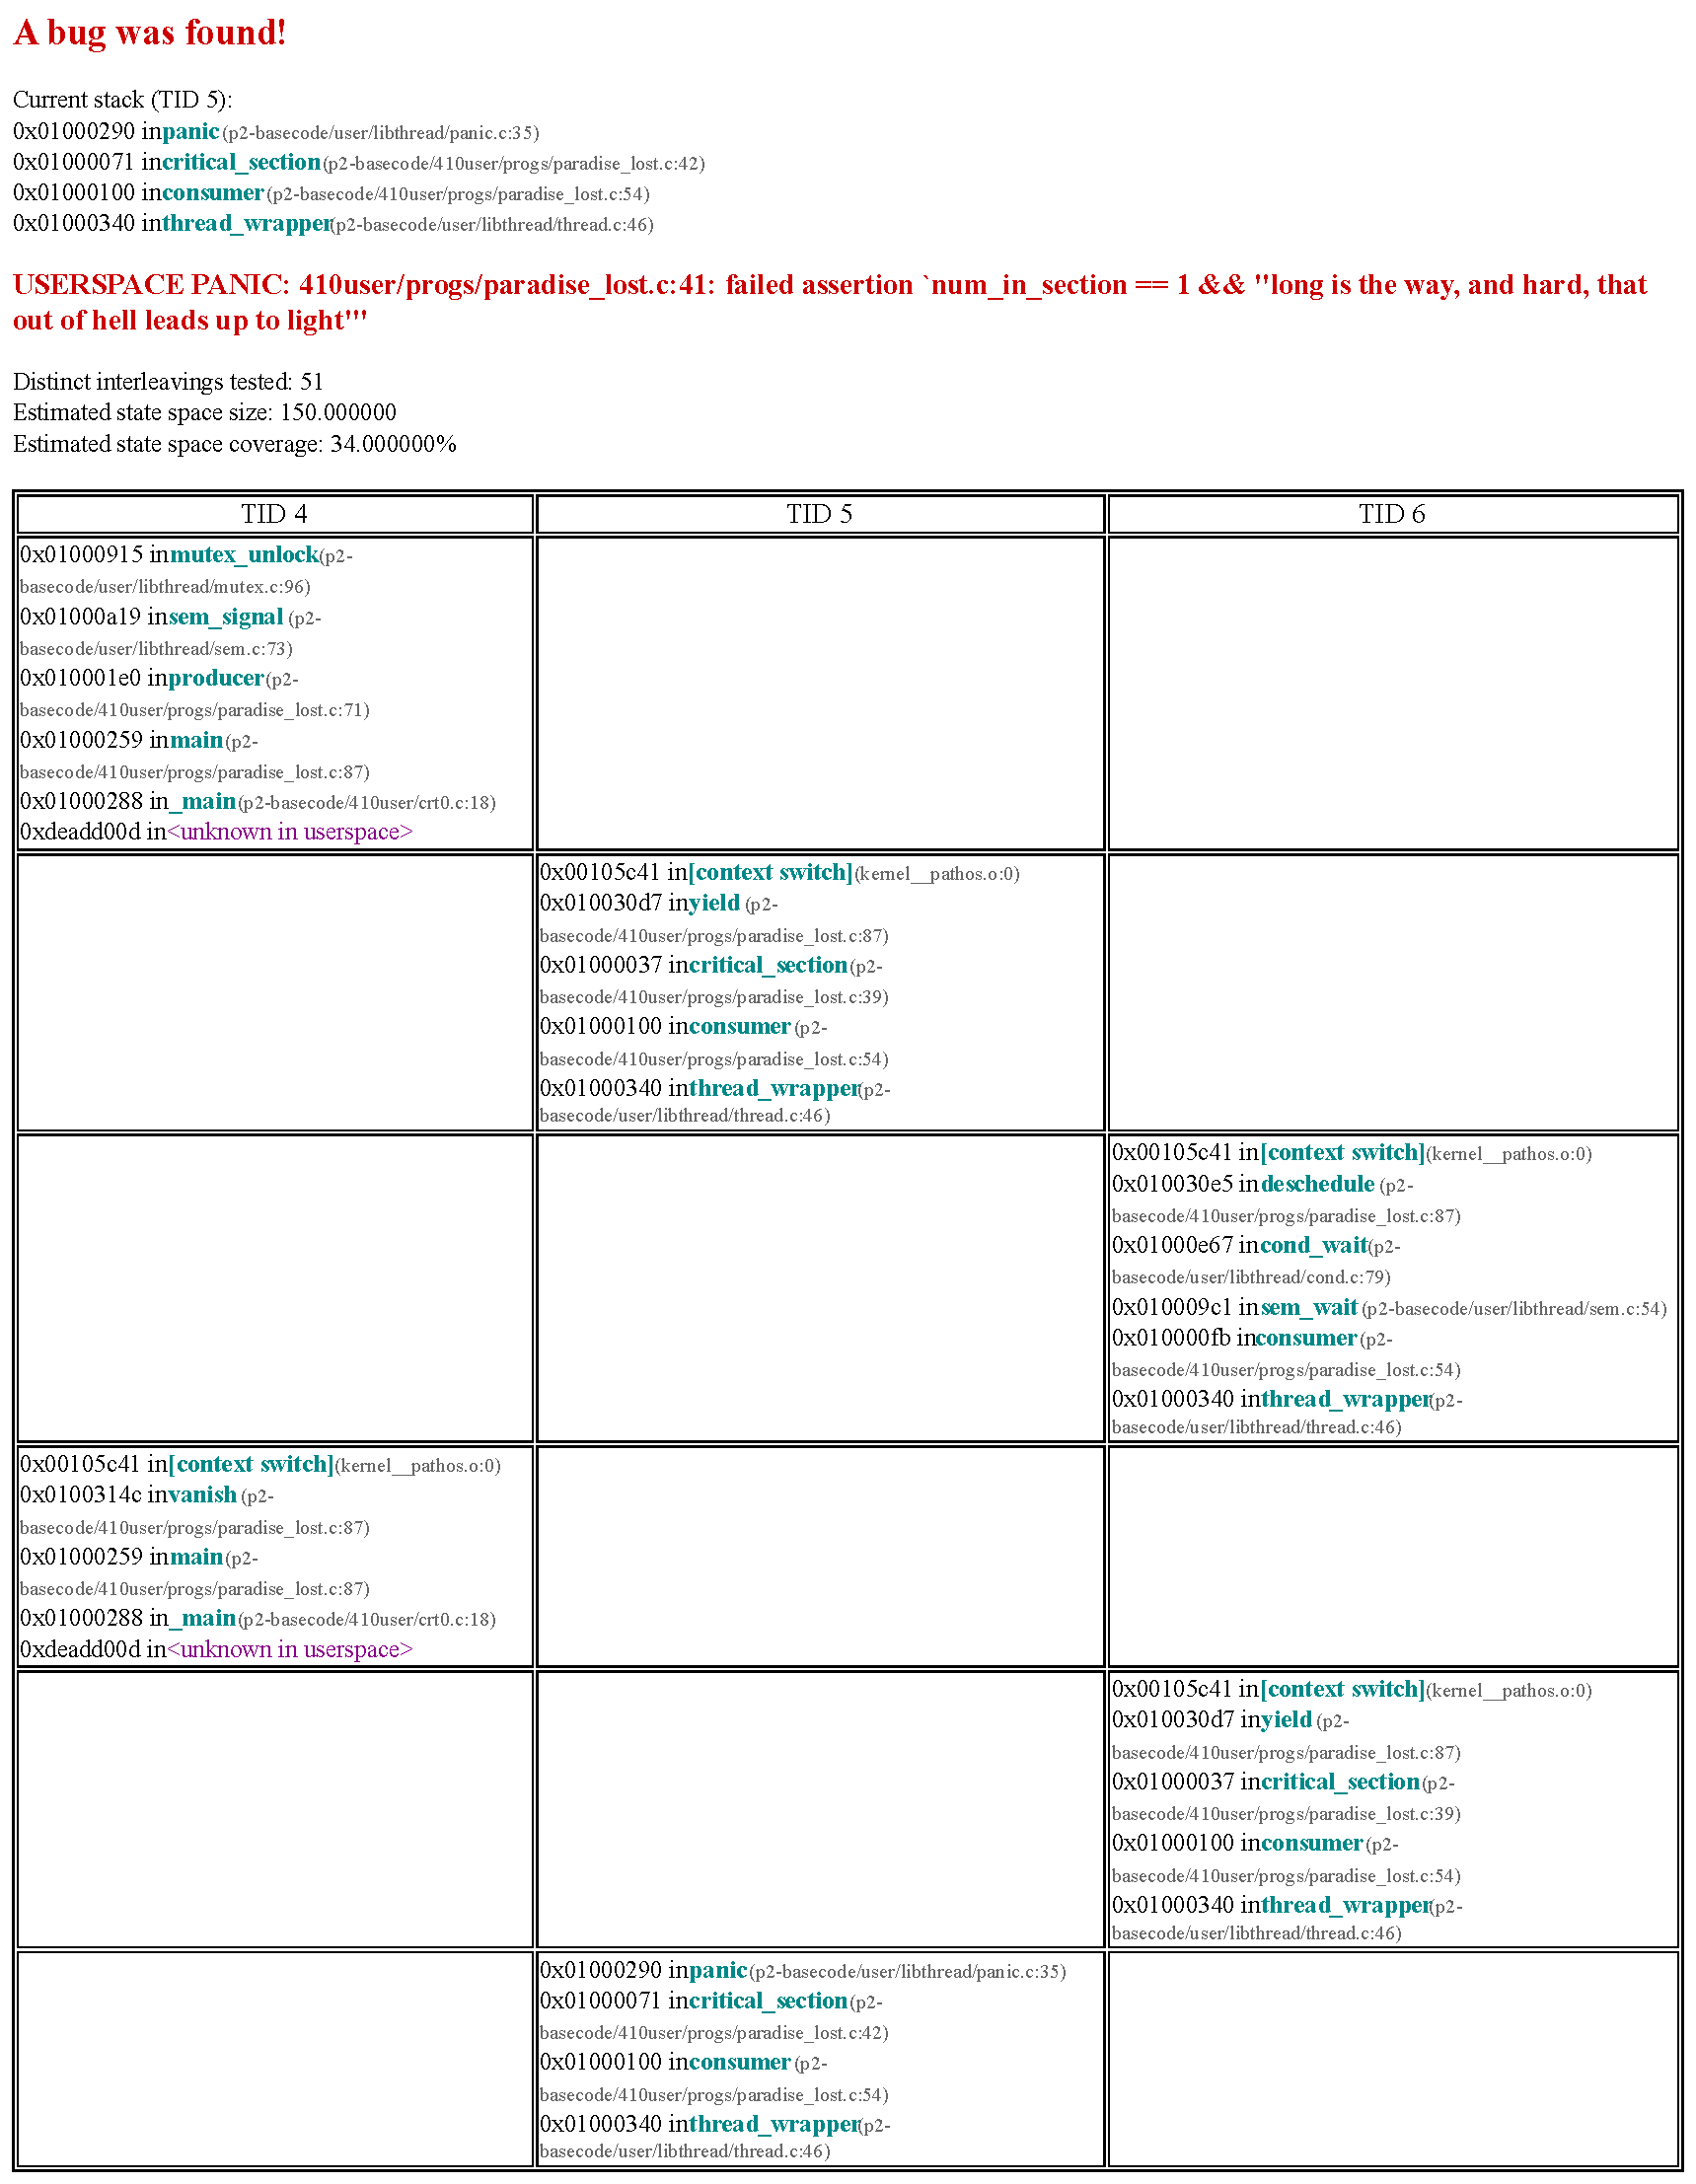
\includegraphics[width=\textwidth]{bugreport.pdf}
	\end{center}
	\caption{Example preemption trace bug report.}
	\label{fig:bugreport}
\end{figure}

%%%%%%%%%%%%%%%%%%%%%%%%%%%%%%%%%%%%%%%%%%%%%%%%%%%%%%%%%%%%%%%%%%%%%%%%%%%%%%%%
%%%%%%%%%%%%%%%%%%%%%%%%%%%%%%%%%%%%%%%%%%%%%%%%%%%%%%%%%%%%%%%%%%%%%%%%%%%%%%%%
%%%%%%%%%%%%%%%%%%%%%%%%%%%%%%%%%%%%%%%%%%%%%%%%%%%%%%%%%%%%%%%%%%%%%%%%%%%%%%%%

\section{Kernel annotations}

The educational experiments in this thesis focus on projects which students implement on top of provided kernel basecode which Landslide already ``understands''.
Such understanding is conferred via the annotations described in this section.
For P2 and Pintos students I supply these annotations behind the scenes,
but a CMU 15-410 student who wishes to use Landslide on their kernel project shall need to brave forth hereupon.

%%%%%%%%%%%%%%%%%%%%%%%%%%%%%%%%%%%%%%%%%%%%%%%%%%%%%%%%%%%%%%%%%%%%%%%%%%%%%%%%

\subsection{config.landslide annotations}
\label{sec:landslide-config-landslide}

The following annotations are specified in {\tt pebsim/config.landslide} akin to the static configuration options
described in \sect{\ref{sec:landslide-directly}}..
These specify the names of kernel functions, global variables, default values, and so on
which are required to accurately track the kernel's scheduler state:
{\tt CONTEXT\_SWITCH},
{\tt EXEC},
{\tt FIRST\_TID},
{\tt IDLE\_TID},
{\tt INIT\_TID},
{\tt MEMSET},
{\tt PAGE\_FAULT\_WRAPPER},
{\tt READLINE},
{\tt SFREE},
{\tt SHELL\_TID},
{\tt SPURIOUS\_INTERRUPT\_WRAPPER},
\\
{\tt THREAD\_KILLED\_ARG\_VAL},
{\tt THREAD\_KILLED\_FUNC},
{\tt TIMER\_WRAPPER},
{\tt VM\_USER\_COPY},
\\
{\tt VM\_USER\_COPY\_TAIL},
{\tt YIELD}.

Following are the less self-explanatory options.
\begin{itemize}
	\item {\tt PINTOS\_KERNEL=0} - configure Landslide for Pebbles (0) or Pintos (1) kernel architecture. Normally set automatically by the setup scripts.
	\item {\tt TESTING\_USERSPACE=1} - configure Landslide whether to test (i.e., focus preemption points, memory analysis, etc. on) the userspace or kernelspace code.
	\item {\tt CURRENT\_THREAD\_LIVES\_ON\_RQ=0} - Landslide infers the list of runnable threads from the {\tt tell\_landslide\_on\_rq()} and {\tt off\_rq()} annotations (described below).
		Some kernels\footnote{most, actually} remove the current thread from their runqueue,
		such that the abstract set of all runnable threads is actually the runqueue plus the current thread rather than just the runqueue.
		Other kernels\footnote{the author's own student kernel from long ago}
		leave the current thread on the runqueue,
		removing it only when it's descheduling and should actually be considered blocked.
		Set this option to 0 to support the former kernel type or 1 to support the latter.%
		\footnote{This option replaces the deprecated {\tt kern\_current\_extra\_runnable()} annotation from {\tt student.c} described in \cite{landslide} \S{}6.2.3.}
	\item {\tt PREEMPT\_ENABLE\_FLAG=NAME} - name of a global variable which the kernel uses to toggle scheduler preemptability, for kernels which may disable preemption without disabling interrupts.
		For kernels wherein preemptability is corresponds directly by interrupts, leave this option unspecified.
	\item {\tt PREEMPT\_ENABLE\_VALUE=VAL} - value of the above variable when preemption is enabled
		(usually 0; note that many kernels use a nesting depth counter where any positive value corresponds to disabled).%
		\footnote{These two options replace the deprecated {\tt kern\_ready\_for\_timer\_interrupt()} annotation from {\tt student.c} described in \cite{landslide} \${}6.2.3.}
	\item {\tt PATHOS\_SYSCALL\_IRET\_DISTANCE=VALUE} - indicate how much stack space is used by the reference kernel's system call wrappers.
		Used for cross-kernel-to-userspace stack traces;
		if unset, stack traces from kernel space will end at the system call boundary.
	\item {\tt PDE\_PTE\_POISON=VALUE} - indicate a poison value used in the page tables to indicate absent VM mappings to check for as well as checking the present bit (if unspecified, will check present bit only)
	\item {\tt BUG\_ON\_THREADS\_WEDGED=1} - set to 0 to disable deadlock detection but instead let the kernel keep receiving system interrupts when all threads appear blocked.%
		\footnote{once used in the bad old days; now recommended for debugging use only}
	\item {\tt TIMER\_WRAPPER\_DISPATCH=NAME} - used to manually indicate a label before the end of the timer interrupt assembly wrapper, in case the {\tt iret} instruction couldn't be found automatically (see {\tt pebsim/definegen.sh}).
	\item {\tt starting\_threads TID STARTS\_ON\_RQ} - specifies a system thread which already exists at the time {\tt tell\_landslide\_sched\_init\_done()} (see below) is called; {\tt TID} is the thread's ID and {\tt STARTS\_ON\_RQ} is 0 or 1 to indicate whether or not it starts on the system runqueue.
		Typical threads to use this for are init and idle.
	\item {\tt ignore\_sym NAME SIZE} - specifies a global variable {\tt NAME} of a given {\tt SIZE} in bytes whose memory accesses should be ignored for the purposes of DPOR and data race analysis.
		Typical symbols to use this for are the console or heap mutex.
	\item {\tt sched\_func NAME} - specifies a function whose memory accesses should all be ignored for the purposes of DPOR and data race analysis.
		Typical functions to use this for are the timer handler and context switcher.
	\item {\tt disk\_io\_func NAME} - specifies a function which may block a thread waiting for disk I/O (or other external interrupt) rather than blocking on another thread.
		If any threads are blocked in a disk I/O function during an apparent deadlock,
		Landslide will allow the kernel to idle until the simulator delivers the appropriate interrupt,
		rather than declaring a bug.
	\item {\tt ignore\_dr\_function NAME USERSPACE} - specifies a function whose memory access should not be counted as data races (but still be considered memory conflicts for DPOR).
		{\tt USERSPACE} should be 0 or 1 to denote a kernel-space or user-space function respectively.
\end{itemize}

%%%%%%%%%%%%%%%%%%%%%%%%%%%%%%%%%%%%%%%%%%%%%%%%%%%%%%%%%%%%%%%%%%%%%%%%%%%%%%%%

\subsection{In-kernel code annotations}

The following annotations are provided as C functions
which a kernel author shall include in their source code and call at appropriate times.
The functions' actual implementations are empty;
rather they serve as labels whose positions the annotation scripts extract
along with the other various annotations from the previous section.
Some of these are mandatory for Landslide to function properly,
while others serve to improve or otherwise manipulate the state space.

\subsubsection{Mandatory annotations}

\begin{itemize}
	\item {\tt tell\_landslide\_thread\_switch(int new\_tid)} - to be called during context switch, indicating the newly-running thread
		(must be called with interrupts and/or scheduler preemption disabled)
	\item {\tt tell\_landslide\_sched\_init\_done()} - to be called after scheduler initialization,
		indicating the point after which Landslide should begin analysis.
		Any threads already initialized before this point (init, idle, etc) should be specified with {\tt starting\_threads} (previous subsection).
	\item {\tt tell\_landslide\_forking()} - to be called whenever a new thread is created,
		``immediately'' before the next {\tt thread\_switch()} or {\tt on\_rq()} call for that new thread (i.e., this call sets a flag which the next instance of either of the latter will check to see if the indicated thread is new).
		Most Pebbles kernels will call this twice; once in {\tt fork} and once in {\tt thread\_fork}.
	\item {\tt tell\_landslide\_vanishing()} - to be called whenever a thread ceases to exist,
		``immediately'' before the next {\tt thread\_switch()} or {\tt off\_rq()} call for the exiting thread
		(works similarly to above).
	\item {\tt tell\_landslide\_sleeping()} - to be called whenever a thread is about to {\tt sleep()} waiting for timer interrupts,
		``immediately'' before the next {\tt thread\_switch()} or {\tt off\_rq()} call for the sleeping thread
		(similar to the above).
		Landslide considers sleeping threads to be runnable as normal (they will just take more timer interrupts to arrive at),
		so this call is necessary to distinguish from the case when a thread is descheduled on a non-timer event.
	\item {\tt tell\_landslide\_thread\_on\_rq(int tid)} - to be called when a thread is added to the runqueue
		(must be called with interrupts and/or scheduler preemption disabled).
	\item {\tt tell\_landslide\_thread\_off\_rq(int tid)} - dual of the above.
		If {\tt CURRENT\_THREAD\_\allowbreak{}LIVES\_ON\_RQ=0} (described above), this should be invoked (among other times) during context switch with the TID of the thread about to start running.
		Alternatively (thanks sully), even for a kernel which takes the current thread off its literal runqueue,
		the annotator may use these two calls to indicate the ``abstract runqueue'' which includes the current thread as well,
		and set {\tt CURRENT\_THREAD\_LIVES\_ON\_RQ=1}.
\end{itemize}

\subsubsection{Optional annotations}

\begin{itemize}
	\item {\tt tell\_landslide\_preempt()} - specifies a preemption point.
		Subject to the constraints of {\tt within\_function}/{\tt without\_function};
		hence may be ignored if used with Quicksand.
	\item {\tt tell\_landslide\_dump\_stack()} - instructs Landslide to print a stack trace whenever this point is reached (for debugging purposes).
\end{itemize}

\subsubsection{Optional but strongly recommended annotations}

The following annotations enable Landslide to track locksets for data race analysis.
If not provided, it will be as if Landslide assumes no guarantees about mutual exclusion or happens-before,
and hence will identify all memory conflicts as data races.
(Note that the corresponding instrumentation for P2s is achieved automatically,
as the names of the mutex interface are mandated by the project specification.)

\begin{itemize}
	\item {\tt tell\_landslide\_mutex\_locking(void *mutex\_addr)} - indicates the beginning of the lock routine for
		whatever synchronization API Landslide should treat as the primitive for data race detection.
		In Pintos this is the {\tt sema\_*()} function family; in Pebbles they may be called anything.
	\item {\tt tell\_landslide\_mutex\_blocking(int owner\_tid)} - called ``immediately'' before a thread becomes blocked on the mutex.
		Definition of ``immediately'' similar to the {\tt forking()} and friends annotations above.
		{\tt owner\_tid} allows Landslide to efficiently unblock/re-block threads when the mutex holder changes
		(rather than relying on heuristic yield-loop detection);
		see {\tt kern\_mutex\_block\_others()} and {\tt deadlocked()} in {\tt schedule.c} for implementation details.
	\item {\tt tell\_landslide\_mutex\_locking\_done(void *mutex\_addr)} - indicates the end of the lock routine.
	\item {\tt tell\_landslide\_mutex\_trylocking(void *mutex\_addr)} - indicates the beginning of the trylock routine (if present).
	\item {\tt tell\_landslide\_mutex\_trylocking\_done(void *mutex\_addr, int succeeded)} -
		indicates when a thread is finished trylocking, even if it failed to get the lock (indicated by {\tt succeeded}).
	\item {\tt tell\_landslide\_mutex\_unlocking(void *mutex\_addr)} - indicates the beginning of the unlock routine.
	\item {\tt tell\_landslide\_mutex\_unlocking\_done()} - indicates the end of the unlock routine.
\end{itemize}

%%%%%%%%%%%%%%%%%%%%%%%%%%%%%%%%%%%%%%%%%%%%%%%%%%%%%%%%%%%%%%%%%%%%%%%%%%%%%%%%
%%%%%%%%%%%%%%%%%%%%%%%%%%%%%%%%%%%%%%%%%%%%%%%%%%%%%%%%%%%%%%%%%%%%%%%%%%%%%%%%
%%%%%%%%%%%%%%%%%%%%%%%%%%%%%%%%%%%%%%%%%%%%%%%%%%%%%%%%%%%%%%%%%%%%%%%%%%%%%%%%

\section{Architecture}

This section documents the organization of code within Landslide.
Unless otherwise specified, Landslide's code lives in
%C files live in
{\tt work/modules/landslide/} (Simics implemenation) or {\tt src/bochs-2.6.8/instrument/landslide/} (Bochs implementation)
relative to the repository root.

Both simulators invoke Landslide once per instruction and once per memory read or write.
% just before..
The entry point is the aptly-named {\tt landslide\_entrypoint()} in {\tt landslide.c},
which then dispatches to various other modules their respective analyses, described as follows.

%%%%%%%%%%%%%%%%%%%%%%%%%%%%%%%%%%%%%%%%%%%%%%%%%%%%%%%%%%%%%%%%%%%%%%%%%%%%%%%%

\subsection{Execution Tree}
\label{sec:landslide-save}

The execution tree
%(or state space, or preemption point log, however calling it suits you)
is stored as a chain of preemption point nodes named {\tt struct hax} defined in {\tt tree.h}.
Although the state space of possible interleavings is exponentially-sized,
Landslide does not actually need to store any nodes for execution sequences outside the current variation
(see \sect{\ref{sec:landslide-estimate}} and \sect{\ref{sec:landslide-dpor}} for why),
so the total memory consumption is only $O(n)$ in the number of preemption points in a single program run
(for the test cases used in this thesis, typically 20-1000).
Each {\tt hax} stores the following information:

\begin{itemize}
	\item Basic statistics such as the current instruction pointer, thread ID,
		stack trace of current thread at the moment of preemption,
		depth in the tree, parent node pointer, etc.;
	\item Snapshots of the current state of the scheduler (\sect{\ref{sec:landslide-scheduler}})
		and memory accesses and heaps (\sect{\ref{sec:landslide-memory}});
	\item Simulator-dependent data needed to time travel and resume execution
		from this checkpoint (\sect{\ref{sec:landslide-timetravel}});
	\item List of parent/ancestor nodes with memory conflicts and/or happens-before edges to this one
		for DPOR (\sect{\ref{sec:landslide-dpor}});
	\item Current estimated state space proportion and execution time for the subtree rooted at this node
		(not necessarily fully explored yet) for estimation \sect{\ref{sec:landslide-estimate}};
	\item Whether this point is an {\tt xbegin} invocation
		and if so what {\tt xabort} codes are possible and/or already explored for this transaction
		(\sect{\ref{chap:txn}}).
\end{itemize}

%%%%%%%%%%%%%%%%%%%%%%%%%%%%%%%%%%%%%%%%%%%%%%%%%%%%%%%%%%%%%%%%%%%%%%%%%%%%%%%%

\subsection{Scheduler}
\label{sec:landslide-scheduler}

The Landslide scheduler, which lives in {\tt schedule.c}, has two main duties:
to maintain an accurate representation of all the existing threads on the simulated system
and track what concurrency-relevant actions each is performing at any given time,
and to orchestrate the sequence of timer interrupts necessary
to cause the simulated system to context switch to any given thread at any given time.
System-wide state is stored in a single {\tt struct sched\_state},
including the thread queues (runqueue, deschedule queue, and sleep queue),
while per-thread state is stored in {\tt struct agent}s (named after the terminology of \cite{dbug-ssv}) which live on said queues.

It has one main entrypoint, {\tt sched\_update()}, in which both the state machine is updated and scheduling decisions are made.
The interface also offers helper functions for finding and manipulating {\tt agent}s,
and {\tt sched\_recover()}, which prepares the scheduler to force a new thread to run
after a time travel (\sect{\ref{sec:landslide-timetravel}}).

\subsubsection{State machine}

The first part of {\tt sched\_update()} is to update the state machine of thread actions and runnability.
Much of this functionality is found in
{\tt sched\_update\_kern\_state\_machine()}
and
{\tt sched\_update\_user\_state\_machine()}.
The current intruction pointer is compared against the known locations of
the mutex API, system calls, runnable/descheduling {\tt tell\_\allowbreak{}landslide} annotations, and so on,
and locksets, action flags, and runqueue membership are updated accordingly.

\subsubsection{Interrupt injection}

The second part of {\tt sched\_update()},
conditional on the arbiter identifying preemption points (\sect{\ref{sec:landslide-arbiter}}),
manages timer interrupts to switch to a desired thread.
Whenever a preemption point is reached,
the scheduler first creates a checkpoint in the execution tree (\sect{\ref{sec:landslide-save}}),
asks the arbiter which thread to run next,
and if that thread is different from the current one,
forces the kernel into its timer interrupt handler (\sect{\ref{sec:landslide-interrupce}}).

Because the kernel is part of the system being tested, Landslide can't necessarily always switch directly to a specific thread,
but rather must keep triggering context switches until the desired thread is reached;
any mechanism to tell the kernel which thread we want would necessarily involve modifying the code being testsed
and hence possibly obscuring bugs or introducing new ones.%
\footnote{For userspace testing, where I supply a pre-annotated reference kernel,
such an approach would be more straightforward,
but the kernel-testing repeated-context-switch approach infrastructure was already in place
and it was easier to reuse that than to add more code.}

The scheduler marks up to one thread as the ``schedule target'',
which when set makes Landslide wait until that thread is reached before looking for more preemption points,
so the kernel may finish its context switches undisturbed.
Whenever the schedule target is set and the end of the context switcher is reached,
if the schedule target is not the current thread,
the scheduler repeats this process until it is.%
\footnote{Note that this ``loop'' is not structured as an explicit loop in Landslide's code,
but rather as part of the state machine which updates each time a new instruction is traced.}

%%%%%%%%%%%%%%%%%%%%%%%%%%%%%%%%%%%%%%%%%%%%%%%%%%%%%%%%%%%%%%%%%%%%%%%%%%%%%%%%

\subsection{Memory analysis}
\label{sec:landslide-memory}

{\tt memory.c} is responsible for all manner of memory access analysis.
It tracks heap allocations, checks reads and writes in the heap region against same;
tracks reads and writes (in any region) from each thread
and checks them against each other
for DPOR (\sect{\ref{sec:landslide-dpor}})
and data race analysis (\sect{\ref{sect:landslide-datarace}}).

\subsubsection{Heap checking}

{\tt mem\_update()} serves as the main entrypoint for tracking heap allocations.
It's called every instruction to check for the boundaries of the {\tt malloc} library,
and behaves in a similar way to the scheduler state machine described above.
Then, {\tt mem\_check\_shared\_access()} checks
(after some elaborate manoeuvres to figure out whether to use the kernel- or userspace heap)
whether, if in the heap region, the memory is contained in a currently-allocated heap block,
reporting a bug if not.

\subsubsection{Memory conflicts}

{\tt mem\_check\_shared\_access()} also records each such access in a per-thread-transition rbtree,
which is saved and then cleared at each preemption point.
This allows {\tt mem\_shm\_\allowbreak{}intersect()}, called at each preemption point once for each of its ancestors
($n^2$ total calls per interleaving),
to perform a set intersection to find any memory conflicts.
Any such conflicts which also fail a lockset
and/or happens-before check (\sect{\ref{sec:landslide-datarace}})
are then reported as data races.
Regardless, all such conflicts are later used by DPOR (\sect{\ref{sec:landslide-dpor}}) to find dependent transition pairs.

%%%%%%%%%%%%%%%%%%%%%%%%%%%%%%%%%%%%%%%%%%%%%%%%%%%%%%%%%%%%%%%%%%%%%%%%%%%%%%%%

\subsection{Machine state manipulation}

The interface to inspect and manipulate the simulated machine state lives in {\tt x86.c}.

\subsubsection{Memory}

{\tt read\_memory()} and {\tt write\_memory()} are both provided (with various wrapper macros in {\tt x86.h}).
The former is used basically everywhere throughout Landslide to query the machine state;
the latter is used only by the interrupt manipulation below
and by the scheduler to force Pintos to skip certain parts of its init sequence (\sect{\ref{sec:landslide-pintosspecifics}}).
Both rely on the helper function {\tt mem\_translate()} for virtual address resolution,
which at present supports only the normal x86 32-bit addressing mode (no PAE, long mode, etc.).

\subsubsection{Interrupts}
\label{sec:landslide-interrupce}

Several routines are provided for manipulating system interrupts.
Note that the Landslide is called once per fetch-decode-execute loop of the CPU,
after the CPU processes all already-pending interrupts and decides which instruction to execute,
but before actually executing the instruction
(true of both Bochs and Simics).
I refer to this as the {\em upcoming instruction}.
Whether or not Landslide wants that instruction to execute before triggering a thread switch is a matter of some concern in the following API.

\begin{itemize}
	\item {\tt cause\_timer\_interrupt()}
		triggers a pending timer interrupt, whose handler will be entered as soon as the upcoming instruction is executed.
	\item {\tt cause\_timer\_interrupt\_immediately()}
		does as above, but forces the system to enter the interrupt handler before the upcoming instruction is executed.
		That instruction will be executed upon return from the interrupt.
	\item {\tt avoid\_timer\_interrupt\_immediately()}
		suppresses a timer interrupt triggered by the simulator from outside of Landslide's control.
		It acknowledges the APIC and forces the system to jump to the end of the interrupt handler.
	\item {\tt delay\_instruction()}
		forces the system to execute a no-op before the upcoming instruction,
		effectively converting an invocation of {\tt cause\_timer\_interrupt()} to {\tt cause\_timer\_interrupt\_immediately()}.
	\item {\tt cause\_keypress()} triggers a keyboard event corresponding to the specified character.
		The interrupt will be taken after the upcoming instruction is executed
		(provided no timer interrupt is simultaneously pending).
		Only {\tt a-z}, {\tt 0-9}, {\tt \_}, space, and newline are supported (enough to name any Pebbles test case).
	\item {\tt interrupts\_enabled()} queries the CPU's interrupt flag ({\tt eflags:IF}).
\end{itemize}

Note that {\tt kern\_ready\_for\_timer\_interrupt()} should generally be invoked separately
from {\tt interrupts\_enabled()} if needed;
while {\tt interrupts\_enabled()} must be true before invoking {\tt cause\_timer\_interrupt()},
if the kernel is not ready the interrupt may not be received for a long time.
Also, use of {\tt cause\_timer\_interrupt\_immediately()} must not be used while the kernel is not ready.

%%%%%%%%%%%%%%%%%%%%%%%%%%%%%%%%%%%%%%%%%%%%%%%%%%%%%%%%%%%%%%%%%%%%%%%%%%%%%%%%

\subsection{State space traversal}

Traversal of the state space is implemented in three parts:
first, identifying preemption points when first encountered and selecting which thread to run for its first execution, in {\tt arbiter.c},
second, selecting which preemption point to backtrack to after completing an execution
and which thread to ``have switched to'' %
% TODO: post-revisions; uncomment; change " %" above to "%"
%\footnote{willan on-having switched to \cite{hhgg-reu}}
instead, in {\tt explore.c},
and third, rewinding the machine state to implement said backtracking,
in {\tt timetravel.c} (Bochs version) and {\tt timetravel-simics.c} (Simics version).

\subsubsection{Arbiter}
\label{sec:landslide-arbiter}

The arbiter (named after the corresponding component of dBug \cite{dbug-ssv})
is responsible for checking which code locations during execution should be identified as preemption points
({\tt arbiter\_interested()}),
and thereupon for choosing whether to keep running the current thread or to preempt and switch to a new one
({\tt arbiter\_choose()}).
Its behaviour in the former case is configured by the options listed in \sect{\ref{sec:landslide-dynamicconfig}},
and in the latter case by the options listed in \sect{\ref{sec:landslide-staticconfig}}.
For example, {\tt EXPLORE\_BACKWARDS} is interpreted here;
if set, it will cause Landslide to always preempt and switch threads the first time it encounters each new preemption point.%
\footnote{Another secret option, {\tt CHOOSE\_RANDOMLY},
also exists here to randomize whether to ``explore backwards''
(choosing independently at each preemption point, resulting in an overall unpredictable exploration order).
% TODO: decide whether you're gonna put those estimate graphs in here
%% I
It's not exposed to {\tt config.landslide} but rather the user must edit it in {\tt arbiter.c} directly,
whereupon the probability may also be adjusted via {\tt numerator} and {\tt denominator}.}

\subsubsection{Explorer}

Landslide invokes the explorer at the end of each execution of the test case,
which analyzes the current branch of the interleaving state space tree
to figure out which alternate branch to try executing next.
Its contents are largely algorithmic rather than architectural
and hence further described in \sect{\ref{sec:landslide-dpor}} and \sect{\ref{sec:landslide-icb}}.

\subsubsection{Time Travel}
\label{sec:landslide-timetravel}

After the explorer picks a past point of the program to preempt, % sorry this started out like that and i just had to roll with it
Landslide collaborates with the simulator to revert the machine state to that point before switching to the desired thread.
The Simics version is merely a bunch of wrapper glue code around the {\tt set-bookmark} and {\tt skip-to} backtracking commands.
Bochs however does not support backtracking, so I instead use {\tt fork()} to get Linux to copy the machine state for me.

The big issue to note here is that, while the simulation state should be completely reverted,
parts of Landslide's state (e.g., scheduler runqueues, thread action flags)
should likewise be reverted to mirror the change in program state,
while others (tagged ancestor branches from DPOR, state space estimates) should be preserved from branch to branch.
In Simics, I simply copy every data structure of the former case ({\tt copy\_sched()} and friends in {\tt save.c}),
leaving those of the latter undisturbed across backtracks.%
\footnote{Simics actually wants to save/restore all its modules' internal state on its own,
offering an attribute set/get API for modules to expose such state (used for other purposes in {\tt simics\_glue.c}),
but doing deep copies of data structures this way would be more trouble than it's worth.}

In Bochs, {\tt fork()} automatically copies everything, so the reverse holds:
all data of the latter case must whenever updated be propagaged to all {\tt fork()}ed children processes explicitly.
I worried while implementing this that I might miss a case, or that future updates to the code could easily forget this step,
resulting undoubtedly in state corruption bugs which to diagnose would be a thesis in their own right,
so I enlisted help from my compiler via the oft-ridiculed {\tt const}.
Every preemption point node in the execution tree ({\tt tree.h}),
each of whose state is kept generally read-only,
and all modifications must go through {\tt modify\_hax()} ({\tt timetravel.h}) using a modification callback,
which internally casts away the {\tt const}, performs the requested modification,
and also messages all relevant child processes to perform the same ({\tt timetravel\_set()} in {\tt timetravel.c}).
The {\tt const} is absolutely, inviolably, not to be casted away, at the sacred cost of what little type safety C offers.%
\footnote{Of course this would be followed by a footnote describing the one place where I cast it away anyway,
{\tt mem\_check\_shared\_access()} in {\tt memory.c};
why it's ok is documented in an {\tt XXX} comment in the code.}
Thence the typechecker enforces that all exploration-related state is properly propagated while scheduler state is automatically reverted.

%%%%%%%%%%%%%%%%%%%%%%%%%%%%%%%%%%%%%%%%%%%%%%%%%%%%%%%%%%%%%%%%%%%%%%%%%%%%%%%%

% time travel, explore, arbiter
\subsection{Bug-finding output}

The infrastructure for producing the diagnostic output to help users understand their bugs
can be classified in three parts:
the symbol table glue, the excessively clever stack tracer, and the preemption table generator.

\subsubsection{Symbol table}

The symbol table logic lives in {\tt symtable.c} and is pretty much a lot of glue code.
In the Simics version, Landslide relies on the {\tt deflsym} Simics object created by the 15-410 python scripts,
and queries its attributes using Simics API calls.
In the Bochs version, function names and line numbers are handled separately:
Bochs is patched with a new API function named {\tt bx\_dbg\_symbolic\_address\_landslide}%
\footnote{does the same thing as the existing {\tt bx\_dbg\_symbolic\_address}, but with a better type signature}
which provides function names and hexadecimal offsets;
while for line numbers, {\tt pebsim/pintos/build.sh}%
\footnote{Line numbers in Bochs for Pebbles/P2s are not supported yet; see {\tt p2-setup.sh} for the work-in-progress.}
generates a header file {\tt line\_numbers.h}
using {\tt objdump} and {\tt addr2line},
which the aforementioned hex offset then serves as an index into.

\subsubsection{Stack traces}

The stack tracer is implemented in {\tt stack.c}.
It does the standard approach of following the base pointer chain
(not supporting code compiled with {\tt -fomit-frame-pointer} by doing anything clever
like understanding how much stack frame is allocated for each function),
and printing symbol table information for the pushed return addresses at the top of each frame.

However, it also offers several special-case features
which even some students have sometimes noticed as being more clever than Simics's stack tracer.
I document those features here.
As a common point of implementation among them,
Landslide traces the stack pointer {\tt esp} in addition to the base pointer {\tt ebp};
not only updating it whenever dereferencing the base pointer,
but also when decoding simple assembly routines, finding ``hidden'' stack frames without base pointers,
identifying system call wrappers, and so on.
The corresponding code lives in {\tt stack\_trace()} in {\tt stack.c}.

\begin{itemize}
	\item If a function is preempted at its beginning or end
		such that its corresponding base pointer is missing from the base pointer chain,
		Landslide will find its ``hidden'' frame and include it in the stack trace in the following cases.%
		\footnote{Note that in such cases,
		most other debuggers' stack tracers will be missing not the name of the interrupted function,
		but the name of the function which called that function,
		because it's the former's stack frame which should enable the debugger
		to find the pushed return address for the latter.}
		\begin{itemize}
			\item If the last pushed return address is at offset 0 into the body of its containing function,
				Landslide will find the next pushed return address at {\tt esp+0}.
			\item If as above but the function is the page fault handler, at {\tt esp+4}.
			\item If the return address is at offset 1 and the previous instruction was {\tt push ebp},
				Landslide will find the next pushed return address at {\tt esp+4}.
			\item If the return address is a multiple of 4 offset
				and all previous instructions are of the form {\tt mov m32,r32},
				Landslide will find the next pushed return address at {\tt esp+0}.
				(This is common in student hand-written assembly functions.)
		\end{itemize}
	\item If the instruction at a pushed return address is a {\tt pop} or {\tt popa},
		Landslide will search for the next non-{\tt pop}({\tt a}) instruction,
		and if it's {\tt ret} or {\tt iret},
		treat the function as a system call wrapper
		(which tend not to preserve the base pointer chain)
		and find the next return address above where all those registers were pushed.
	\item If a return address was pushed during a fault or interrupt
		(determined by checking for the {\tt iret} opcode or the page fault wrapper special case mentioned above),
		Landslide will read the iret block to determine whether a stack switched happened
		and if so what {\tt esp} used to be.
	\item If a return address's offset into its containing function is 0,
		and the last instruction in the preceding function (binary-wise) is a {\tt call},
		Landslide will recognize it as a {\tt noreturn} tail-call, and print the correct function name.%
		\footnote{Normally Landslide reports function/line number information for the return address as-is,
		which indicates the next line of code after the relevant call rather than the call itself.}
	\item Landslide runs the tortoise/rabbit algorithm to detect cyclic {\tt ebp} chains and terminate after the first time around.
	\item Two other Pebbles-specifc special cases described in \sect{\ref{sec:landslide-pebblesspecifics}}.
\end{itemize}

Also implemented in {\tt stack.c} is the backend of the {\tt within\_function}/{\tt without\_function} configuration command,
which searches a given stack trace for the presence of a function return address within a specified range.

\subsubsection{Preemption traces}

The preemption traces, described and exemplified in \sect{\ref{sec:landslide-bugreport}}, are generated by {\tt found\_a\_\allowbreak{}bug.c},
in cooperation with {\tt save.c}.
Whenever {\tt save.c} creates a preemption point, it captures a stack trace of the current thread at the point it was interrupted, and saves it in the preemption point tree.
{\tt found\_a\_bug.c} then traverses the current branch of the tree,
potentially producing both console output and HTML output (controlled by the {\tt HTML\_PRINTF} macro family).
It should be invoked by the {\tt FOUND\_A\_BUG} macro defined in {\tt found\_a\_bug.h},
or by {\tt FOUND\_A\_BUG\_HTML\_INFO}, which also allows the caller to specify a callback to print extra details (such as use-after-free stack traces) in the bug report.

%%%%%%%%%%%%%%%%%%%%%%%%%%%%%%%%%%%%%%%%%%%%%%%%%%%%%%%%%%%%%%%%%%%%%%%%%%%%%%%%

\subsection{Pebbles-specific features}
\label{sec:landslide-pebblesspecifics}

This section lists special cases of instrumentation specific to the Pebbles kernel.

\begin{itemize}
	\item {\tt mem\_check\_shared\_access()} ({\tt memory.c})
		will assert that kernel memory is direct-mapped.
	\item {\tt use\_after\_free()} ({\tt memory.c})
		will ignore use-after-free reads originating from kernel code during the {\tt swexn} system call
		(an extremely common and neither harmful nor technically interesting bug among student implementations).
	\item {\tt cause\_test()} ({\tt test.c})
		will issue keyboard input to type the test case name and press enter
		when the initialization sequence completes and the shell is blocked on {\tt readline}.
	\item {\tt kern\_mutex\_block\_others()} ({\tt schedule.c})
		will handle the special ``blocked on via mutex'' state changes
		whenever a mutex is acquired or released,
		for kernels which use the {\tt tell\_landslide\_kern\_mutex\_blocking()} annotation.
	\item {\tt sched\_update\_kern\_state\_machine()} ({\tt schedule.c})
		will handle the reference kernel's invocation of {\tt sched\_unblock()} within {\tt cond\_\allowbreak{}signal()}
		as a signal event for happens-before analysis.
	\item {\tt cause\_timer\_interrupt\_immediately()} ({\tt x86.c})
		will read the {\tt esp0} value out of the TSS to support user-to-kernel mode switches
		in timer interrupts injected during userspace execution.
	\item {\tt splice\_pre\_vanish\_trace} ({\tt stack.c})
		will, when a {\tt vanish}ing thread has already deleted its Simics symbol table object,
		splice in a saved ``pre-vanish'' stack trace
		(saved previously in {\tt sched\_update\_kern\_state\_machine()})
		so the user can see the userspace execution sequence preceding the {\tt vanish} invocation.
	\item {\tt stack\_trace} ({\tt stack.c})
		will, when {\tt ebp} crosses from kernel- to userspace across a system call boundary
		(a reference kernel feature to allow Simics stack traces to cross same),
		use {\tt PATHOS\_SYSCALL\_IRET\_DISTANCE} (\sect{\ref{sec:landslide-config-landslide}})
		to track {\tt esp}'s value across the stack switch.
\end{itemize}

%%%%%%%%%%%%%%%%%%%%%%%%%%%%%%%%%%%%%%%%%%%%%%%%%%%%%%%%%%%%%%%%%%%%%%%%%%%%%%%%

\subsection{Pintos-specific features}
\label{sec:landlside-pintosspecifics}

This section lists special cases of instrumentation specific to the Pintos kernel.

\begin{itemize}
	\item {\tt arbiter\_interested()} ({\tt arbiter.c})
		will automatically insert preemption points on {\tt intr\_disable()} and {\tt intr\_enable()} calls
		(immediately before and after the interrupt state is changed, respectively)
		(as long as they aren't part of the mutex implementation, which has preemption points of its own).
	\item {\tt lockset\_remove()} ({\tt lockset.c})
		will warn instead of panic if a lock is unlocked twice,
		to allow for double {\tt sema\_up()} in cases where the lock is actually a multi-use semaphore rather than a mutex.
	\item {\tt build.sh} will edit the {\tt bootfd.img} binary to implant the name of the test case to be run in the kernel's boot command.
	\item {\tt sched\_check\_pintos\_init\_sequence()} ({\tt schedule.c})
		will force the kernel to skip the {\tt timer\_calibrate()} and {\tt timer\_msleep()} routines
		used in I/O initialization.
	\item {\tt keep\_schedule\_inflight()} ({\tt schedule.c})
		will detect when an attempted thread switch is impossible
		because the timer handler's try-lock will fail,
		and will abort the interleaving early as if it never existed (which it shouldn't).
	\item {\tt sched\_update\_kern\_state\_machine()} ({\tt schedule.c})
		will:
		\begin{itemize}
			\item track invocations of {\tt timer\_sleep()} and {\tt list\_insert\_ordered()}
				to infer when a thread is sleeping rather than blocked automatically,
				rather than relying on the {\tt tell\_landslide\_sleeping()} annotation.
			\item allow {\tt sema\_up()} to reenter itself,
				which may happen when an IDE interrupt is taken when interrupts are re-enabled at the end of said function.
			\item handle interrupt disabling/enabling as an abstract global lock for the purposes of happens-before analysis.
		\end{itemize}
	\item {\tt sched\_update()} ({\tt schedule.c})
		will handle ``lock handoff'' of the abstract disable-interrupts lock
		during a context switch for happens-before analysis.
	\item {\tt memory.c} (various functions)
		will handle page allocations from the {\tt palloc} family of functions in a separate memory heap,
		allowing the usual allocator {\tt malloc} to allocate and free from {\tt palloc}'ed memory,
		and checking both allocation heaps when checking for use-after-frees.
	\item {\tt kern\_address\_in\_heap()} ({\tt kernel\_specifics.c})
		will ignore DMA accesses to the VGA console,
		which appear to be in Pintos's heap region.
	\item {\tt test\_update\_state()} ({\tt test.c})
		will use the boundaries of {\tt run\_test()} to denote the test lifecycle.
\end{itemize}

%%%%%%%%%%%%%%%%%%%%%%%%%%%%%%%%%%%%%%%%%%%%%%%%%%%%%%%%%%%%%%%%%%%%%%%%%%%%%%%%

\subsection{Handy scripts}
\label{sec:landslide-glue}

The options specified in \sect{\ref{sec:landslide-directly}}
are handled by a family of gross shell scripts that live in {\tt pebsim/}.

\begin{itemize}
	\item {\tt landslide} is the outermost script invoked by Quicksand (or by a \sect{\ref{sec:landslide-directly}} aficionado).
		It exports several key environment variables used by the other scripts,
		ensures the instrumentation is up-to-date,
		and launches the simulator.
	\item {\tt getfunc.sh} defines several functions commonly used by {\tt build.sh} and {\tt definegen.sh} to extract function or global variable addresses from the program binary.
	\item {\tt symbols.sh} defines the names of kernel functions that can be instrumented automatically without a corresponding manual annotation (e.g., {\tt malloc} and friends, the names of the {\tt tell\_landslide} family, various library helpers such as {\tt panic}).
	\item {\tt build.sh} ensures the build of Landslide is up-to-date,
		and processes any dynamic configuration options which don't require updating the build (\sect{\ref{sec:landslide-dynamicconfig}})
		It verifies all required {\tt tell\_landslide} annotations are present,
		verifies all required {\tt config.\allowbreak{}landslide} options,
		processes the dynamic config options,
		checks whether or not {\tt definegen.sh} needs to be run again (via hashes stored in {\tt student\_specifics.h} of the program binary and static config options),
		and does so if necessary.
	\item {\tt definegen.sh} produces the
		%automatically-generated
		content of {\tt student\_specifics.h}.
		It repeatedly invokes the helpers defined in {\tt getfunc.sh}
		to find the addresses of both functions specified in the config options
		and functions whose names are known in advance.%
		\footnote{You might think it should invoke objdump but once and keep the output in a shell variable,
		but I tried that and it was mysteriously slower, so I gave up without ever figuring out why.}
\end{itemize}

The final output of these scripts is an auto-generated header, {\tt student\_specifics.h},
containing a bunch of {\tt \#define}s of the addresses of important functions in the compiled binary,
specific features enabled or disabled by the static config options (\sect{\ref{sec:landslide-staticconfig}}),
and so on.
The files {\tt kernel\_specifics.c}, {\tt user\_specifics.c}, and {\tt student.c} provide several interface functions
for interpreting the current program state with respect to these values.

%%%%%%%%%%%%%%%%%%%%%%%%%%%%%%%%%%%%%%%%%%%%%%%%%%%%%%%%%%%%%%%%%%%%%%%%%%%%%%%%
%%%%%%%%%%%%%%%%%%%%%%%%%%%%%%%%%%%%%%%%%%%%%%%%%%%%%%%%%%%%%%%%%%%%%%%%%%%%%%%%
%%%%%%%%%%%%%%%%%%%%%%%%%%%%%%%%%%%%%%%%%%%%%%%%%%%%%%%%%%%%%%%%%%%%%%%%%%%%%%%%

\section{Algorithms of note}

% not worth discussing?
%\subsection{Kernel annotations}
%\subsection{Bug identification}

%%%%%%%%%%%%%%%%%%%%%%%%%%%%%%%%%%%%%%%%%%%%%%%%%%%%%%%%%%%%%%%%%%%%%%%%%%%%%%%%

\subsection{Preemption point identification}
\label{sec:landslide-pps}
% TODO: talk about how w/in func and w/out func are processed
%%%%%%%%%%%%%%%%%%%%%%%%%%%%%%%%%%%%%%%%%%%%%%%%%%%%%%%%%%%%%%%%%%%%%%%%%%%%%%%%

\subsection{State space estimation}
\label{sec:landslide-estimate}
%%%%%%%%%%%%%%%%%%%%%%%%%%%%%%%%%%%%%%%%%%%%%%%%%%%%%%%%%%%%%%%%%%%%%%%%%%%%%%%%

\subsection{Dynamic Partial Order Reduction}
\label{sec:landslide-dpor}

Landslide implements Dynamic Partial Order Reduction (DPOR) \cite{dpor}
to identify concurrent yet independent thread transitions
whose permutations can safely be pruned from the state space
while still testing all possible program behaviours.

The DPOR implementation consists of 3 parts:
computing happens-before,
computing memory conflicts,
and tagging alternate branches to explore to drive the state space exploration.
The former two are computed as each preemption point is reached,
for the associated thread transition pairwise with all other preceding thread transitions.
The latter is computed at the end of each full interleaving executed, using the results of the two former,
and constitutes the bulk of the algorithm.

In this section $t_i$ will denote a transition between two program states during execution,
with each state being a preemption point as identified in \sect{\ref{sec:landslide-pps}},
and $T(t_i)$ will denote the thread which was scheduled to produce that transition.

\subsubsection{Happens-before}

The happens-before relation expresses when two thread transitions can potentially be reordered,
or in other words, are concurrent (despite the serialized nature of the simulated execution).
This relation is expressed in the following definitions paraphrased from \cite{dpor}.

\begin{itemize}
	\item {\bf Enabled}: A transition $t_i$ is enabled in a state $s$ when a state $s'$ exists such that $s \xrightarrow{t_i} s'$ exists.
		In systems terms, the scheduler at state $s$ considers $T(t_i)$ to be runnable.
	\item {\bf Dependent}: Two transitions $t_i$ and $t_j$ are dependent if
		\begin{enumerate}
			\item $t_1$ is enabled in $s$ and $s \xrightarrow{t_1} s'$, and
			\item $t_2$ is enabled in $s$ but not enabled in $s'$, or vice versa.
		\end{enumerate}
		In systems terms, either $T(t_1) = T(t_2)$,
		or the execution of $t_1$ at $s$ causes $T(t_2)$
		to change state from blocked to runnable or vice versa.
		\footnote{The original paper's definition includes a second criterion that, from $s$,
		%the executions $t_1 t_2$ and $t_2 t_1$ result in identical states;
		a state $s'$ exists such that both $s \xrightarrow{t_1 t_2} s'$ and $s \xrightarrow{t_2 t_1} s'$.
		This captures the memory independence relation,
		but computationally requires direct comparison of program states.
		{\em Stateless} model checkers compute memory conflicts separately from happens-before,
		to find and prune such identical states implicitly,
		as described in the next two subsections.}
		Landslide computes this relation in {\tt enabled\_by()} in {\tt save.c}.
	\item {\bf Happens-Before}: The happens-before relation for a transition sequence $S = t_1 \dots t_n$
		is the smallest relation $\rightarrow_S$ on ${1 \dots n}$ such that
		\begin{enumerate}
			\item if $i < j$ and $S_i$ and $S_j$ are dependent then $i \rightarrow_S j$, and
			\item $\rightarrow_S$ is transitively closed.
		\end{enumerate}
		Landslide computes this relation in
		%the aptly-named
		{\tt compute\_happens\_before()} in {\tt save.c}.
\end{itemize}
The happens-before relation is a partial order expressing the scheduling constraints of a given interleaving.
All pairs of interleavings not included are subject to reordering,
and hence candidates for new interleavings to test.

Note that DPOR's notion of happens-before differs from the traditional distributed systems definition \cite{lamport-clocks}
as used in Pure Happens-Before \sect{\ref{sec:background-hb}};
rather, it coincides with condition 3 of Limited Happens-Before %as defined in \sect{\ref{sec:background-datarace}}
(in fact, Landslide's Limited HB implementation simply reuses the same result computed for DPOR's purpose).

\subsubsection{Memory conflicts}

The memory conflict relation expresses when two transitions are dependent,
or in other words, when their behaviour could potentially vary depending which executes first.

Upon execution of each $t_j \in S$,
Landslide saves the current set of all memory accesses since the previous preemption point (call this $M(t_j)$),
compares it to all $M(t_i)$ with $i < j$ and $i \not\rightarrow_S j$,
and then begins recording subsequent memory accesses in a new empty set for $t_{j+1}$.
%When each preemption point is reached,
%Landslide saves the current set of all memory accesses since the previous preemption point,
%compares it to the accesses from all previous transitions by different threads
%which weren't marked as happens-before in the previous section,
%and then empties that set for the next thread transition
({\tt shimsham\_shm()} in {\tt save.c}).
These $M(t)$ sets are mappings from memory addresses to
instruction pointer value, read-or-write boolean, lockset or vector clock, and various other metadata
({\tt struct mem\_lockset} in {\tt memory.h}).

The set intersection is implemented in {\tt mem\_shm\_interseect()} in {\tt memory.c}.
It checks for read/write and write/write pairs to the same address with an $O(\mathsf{max}(m,n))$ scan of both access sets (pre-sorted).
If any address $a$ exists with $a \in M(t_i)$ and $a \in M(t_j)$ and $M(t_i)(a) = \mathsf{write} \vee M(t_j)(a) = \mathsf{write}$
then $t_i$ and $t_j$ are said to conflict,
which I will denote $t_i \leftrightsquigarrow_S t_j$.

Whenever a conflict is identified, it also invokes the data race analysis (\sect{\ref{sec:landslide-datarace}}).
It checks for {\tt free()}/access conflicts as well as access pairs,
effectively treating deallocation of a heap block as a ``poisoning'' write to its entire contents,
which is considered to conflict with accesses to any address therein
on the grounds that reordering may expose a use-after-free.

\subsubsection{State space exploration}

The core of the DPOR algorithm is implemented in {\tt explore()} in {\tt explore.c}.

{\bf Definition.}
Given a transition sequence (execution, interleaving, preemption trace) $S = t_1 \dots t_n$,
the DPOR algorithm identifies any number of alternate interleavings that must be tested.
Each such interleaving I will denote in this section as $I_{ij} = (t_1 \dots t_{i-1}, T_j)$,
where $t_1 \dots t_{i-1}$ is the common execution prefix shared between $S$ and the new interleaving,
and $T_j$ is the thread ID to be scheduled after $t_{i-1}$, $T_j \ne T(t_i)$.
%to run {\em instead} of $T(t_i)$.
\footnote{I describe $T_j$ as a thread ID here, rather than as a thread transition,
because the nature of the transition (its memory accesses, the subsequent state, etc)
is unknown until we actually execute it.}
Landslide's implementation represents $S$ as a list of {\tt struct hax}es, defined in {\tt tree.h},
each one representing a preemption point, or intermediate state between two transitions.

{\bf Identifying new interleavings.}
To summarize, for each pair of transitions $t_i$ and $t_j$ ($i<j$),
DPOR identifies interleavings which will reorder them,
executing $t_j' t_i'$ to reach a new program state not exposed in the current interleaving.
If $t_i \rightarrow_S t_j$ then they cannot be reordered,
and if $t_i \not\leftrightsquigarrow_S t_j$ then reordering them
will produce a state already encountered in this interleaving;
hence, DPOR considers only transition pairs
which are not related by happens-before and are related by memory conflict ({\tt is\_evil\_ancestor()}).

% TODO: change i<4 to i<j.
% i accidentally typed i<4 here and decided it'd be funny to leave it this way
For each such pair $t_i$, $t_j$, $i<4$, let $s$ denote the state (preemption point) immediately before $t_i$.
Then:
\begin{itemize}
	\item If $T(t_j)$ is runnable at $s$, return $I_{ij} = (t_1 \dots t_{i-1}, T_j)$ ({\tt tag\_good\_sibling()}).
	\item Otherwise, there must be some third thread runnable at $s$
		(from $t_i \not\rightarrow_S t_j$, by contrapositive of the second condition of dependence);
		then, return all $I_{ik} = (t_1 \dots t_{i-1}, T_k)$ such that
		$T_k \ne T(t_i)$ and $T_k$ is runnable at $s$
		({\tt tag\_all\_siblings()}).
\end{itemize}

{\bf Tracking already-visited interleavings.}
Let $U(I_{ij})$ denote the sub-state-space (or sub-tree) beginning at the next preemption point reached
after executing $T_j$ after $t_1 \dots t_{i-1}$;
in other words, the set of all sequences $S' = t_1 \dots t_{i-1}, u_i, \dots u_{n'}$ with $T(u_i) = T_j$.
Landslide orders its search depth-first,
so for any such $U$ outside the current interleaving,
either all or none of its $S'$s will have been tested already.
Therefore, to avoid repeating interleavings,
Landslide need only store at each {\tt struct hax} a list of threads
such that their corresponding subtree $U$ is fully explored,
and can omit any non-constant-size information about the contents of that $U$
({\tt struct hax\_child}).
Hence the memory cost of Landslide's DPOR implementation is $O(nk)$,
$k$ being the maximum runnable threads at any preemption point
(which in turn is always single digits for model checking tests).

{\bf Choosing which new interleaving to test next.}
Among all interleavings chosen by DPOR not already marked as explored,
Landslide chooses the one with the longest execution prefix matching the current $S$,
to maintain the depth-first search invariant.
(In the case of a tie, differing only by which thread to run, it chooses arbitrarily.)
All other new interleavings are marked to explore later in their corresponding {\tt struct hax},
and automatically included in the result of any future iterations of DPOR until they are tested.
Because the one with the longest execution prefix was chosen to test next,
all others must share their execution prefixes with it,
preserving the $O(nk)$ memory bound described above.
%so storing markers for the others during the next execution is still $O(1)$ memory.

When DPOR returns no new $I_{ij}$s not already marked in the set of visited subtrees,
the exploration is complete.

\subsubsection{Example}

Acknowledging that quickly gaining an intuitive understanding for an algorithm
is basically impossible from just paragraphs of text,
I provide in this section an example of a single iteration of DPOR
on the example state space from Figures~\ref{fig:concurrency-bug} and \ref{fig:tree}.

%%%%%%%%%%%%%%%%%%%%%%%%%%%%%%%%%%%%%%%%%%%%%%%%%%%%%%%%%%%%%%%%%%%%%%%%%%%%%%%%

\subsection{Data race analysis}
\label{sec:landslide-datarace}

Whenever a memory conflict is identified for DPOR as described above,
the access pair's corresponding locksets and/or happens-before edges are checked to determine if it's also a data race.
Note the distinction: DPOR memory conflicts indicate that two thread transitions,
if reordered, could produce different behaviour, even if all accesses therein are adequately synchronized;
while a data race indicates furthermore that the two threads can be interleaved precisely at the moment of one or both accesses.
% nb. i think "only one of the accesses can be preempted at and have the other interleaved inside, but not the other way around,
% is a property of cli/sti involvement in kernel space only.

The core of the comparison is in {\tt check\_locksets()} in {\tt memory.c}.
It checks each DPOR memory conflict's locksets, for limited happens-before,
and happens-before edges, for pure happens-before
(\sect{\ref{sec:background-hb}}).

\subsubsection{Limited Happens-Before}
\label{sec:landslide-lhb}

Conditions 1, 2, and 4 defined in \sect{\ref{sec:background-hb}}, provided the Limited Happens-Before definition for \#4,
coincide exactly with the conditions to be considered a memory conflict under DPOR.
Hence all that remains to be checked is \#3, the set of locks held by each thread at the time of access.

Routines for recording lockset changes and computing set intersection are found in {\tt lockset.c}.
Apart from standard data structure manipulation,
one algorithmic point of note is that locks are distinguished by types in addition to address.
This allows (e.g.) mutexes stored as part of the implementation of semaphores to protect a different set of accesses than are protected by the semaphore they implement.

% TODO: talk abt free re malloc false positives

\subsubsection{Pure Happens-Before}
\label{sec:landslide-phb}

In Pure Happens-Before,
condition 4 is replaced with the traditional distributed systems notion of Happens-Before \cite{lamport-clocks}.
Landslide implements this via the vector clocks approach described by {\sc FastTrack} \cite{fasttrack}.
I refer the reader interested in the vector clock algorithm itself to the {\sc FastTrack} paper,
limiting discussion here to Landslide's corresponding implementation of each inference rule.

I use the {\sc Djit+} rules for reads and writes rather than the {\sc FastTrack} ones,
even though they more often incur $O(n)$ runtime in the size of the vector clocks:
because Landslide tests should be limited to few threads in order to manage the state space size,
$n$ is always in the single digits, so I optimize for code simplicity.

\begin{itemize}
	\item Reads and writes ({\tt memory.c})
	\begin{itemize}
		\item \textsc{Djit+ read/write same epoch} - {\tt vc\_eq()} case of {\tt add\_lockset\_to\_shm()}
		\item \textsc{Djit+ read/write} - {\tt vc\_happens\_before()} case of {\tt check\_locksets()}
	\end{itemize}
	\item Synchronization ({\tt schedule.c})
	\begin{itemize}
		\item \textsc{FT acquire}
			\begin{itemize}
				\item {\tt kern\_mutex\_\{,try\}locking\_done()} cases of {\tt kern\_update\_state\_\allowbreak{}machine()}
				\item {\tt user\_mutex\_\{,try\}lock\_exiting()} cases of {\tt user\_update\_state\_\allowbreak{}machine()}
				\item {\tt cli} case of {\tt kern\_update\_state\_machine()} (Pintos only)
				\item {\tt cli}/{\tt sti} lock handoff case in {\tt sched\_update()} (Pebbles only)
			\end{itemize}
		\item \textsc{FT release}
			\begin{itemize}
				\item {\tt kern\_mutex\_unlocking()} case of {\tt kern\_update\_state\_machine()}
				\item {\tt user\_mutex\_unlock\_entering()} case of {\tt user\_update\_state\_machine()}
				\item {\tt sti} case of {\tt kern\_update\_state\_machine()} (Pintos only)
				\item {\tt cli}/{\tt sti} lock handoff case in {\tt sched\_update()} (Pebbles only)
			\end{itemize}
		\item \textsc{FT fork} - {\tt agent\_fork()}
		\item \textsc{FT join} - {\tt sched\_unblock()} case of {\tt kern\_update\_state\_machine()}
			(Pebbles only; Pintos case is handled by above {\tt cli}/{\tt sti} cases in context switch)
	\end{itemize}
\end{itemize}

%%%%%%%%%%%%%%%%%%%%%%%%%%%%%%%%%%%%%%%%%%%%%%%%%%%%%%%%%%%%%%%%%%%%%%%%%%%%%%%%

\subsection{Iterative Context Bounding}
\label{sec:landslide-icb}

Iterative Context Bounding \cite{chess-icb} is a state space exploration strategy
that prioritizes interleavings with fewer total preemptions first.
Let $P(I)$ denote the number of preemptions in an interleaving $I$.
Then, to summarize in pseudocode a na\"ive exploration of some state space $S$ as:

\begin{algorithm}[h]
	\ForEach{$I \in S$}{
		Execute($I$)
	}
	\caption{Straightforward exploration ordering}
	\label{alg:not-icb}
\end{algorithm}

% TODO: make sure latex doesn't fuck up the algorithm placement
ICB's approach could likewise be summarized as follows:

\begin{algorithm}[h]
	\For{$n \in [0..\mathsf{max}_P(S)]$}{
		\ForEach{$I \in S, P(I) \le n$}{
			Execute($I$)
		}
	}
	\caption{ICB exploration ordering}
	\label{alg:icb}
\end{algorithm}

%% stupid imperative way to write it
%\begin{algorithm}[h]
%	\For{$n \in [0..\infty]$}{
%		$\mathsf{skipped\_any} := \mathsf{false}$ \\
%		\ForEach{$I \in S$}{
%			\uIf{$P(I) \le n$}{
%				Execute($I$)
%			} \Else {
%				$\mathsf{skipped\_any} := \mathsf{true}$
%			}
%		}
%		\If{$\neg \mathsf{skipped\_any}$}{
%			{\bf Break}
%		}
%	}
%\end{algorithm}

First of all, note that Algorithm~\ref{alg:icb} is structured in a way that repeats interleavings
with fewer than $n$ preemptions that have already been checked in previous iterations of the outer loop.
This is because the number of preemptions in each branch is not known in advance;
rather, the state space must always be explored in an overall depth-first approach,
at best skipping too-preemptful interleavings as they are encountered.
As simple as it would be to state ``{\bf foreach} $I \in {\mathsf{sort}_P(S)}$'' in pseudocode,
implementing such an ordering would be much less straightforward. %
% TODO: post committee review
%\footnote{Translating conference papers' pseudocode into usable implementations is often quite difficult \cite{itg2}.}
The core ICB loop appears in {\tt time\_travel()} in {\tt landslide.c}.
%(although not explicitly structured as a C-style loop in the code)

Secondly, prior work \cite{bpor} has shown that
when combined with DPOR to prune equivalent interleavings,
DPOR's reduction might not be sound with respect to the subset of $S$ under $P \le n$.
That work introduced Bounded Partial Order Reduction (BPOR),
a compatibility extension to DPOR for ICB to address this problem.
To summarize, % TODO: summarize this once you write the DPOR section so you know what terminology to write in terms of
%I refer the reader interested in the algorithm's details to the citation;
%this section will discuss Landslide's implementation.
% TODO: say how u do it

%%%%%%%%%%%%%%%%%%%%%%%%%%%%%%%%%%%%%%%%%%%%%%%%%%%%%%%%%%%%%%%%%%%%%%%%%%%%%%%%

\subsection{Heuristic loop, deadlock, and synchronization detection}
